%miktex
\documentclass[conference]{IEEEtran}

\usepackage{graphicx,times,amsmath,colortbl, psfrag} % Add all your packages here

\usepackage[ruled, vlined, english, boxed, linesnumbered, lined]{algorithm2e} %descargar
\usepackage{algpseudocode} %descargar

\usepackage{multirow}

\usepackage {amsfonts}
\usepackage {amsmath}




% *** GRAPHICS RELATED PACKAGES ***
%
\ifCLASSINFOpdf
  % \usepackage[pdftex]{graphicx}
  % declare the path(s) where your graphic files are
   \graphicspath{{../pdf/}{../jpeg/}}
  % and their extensions so you won't have to specify these with
  % every instance of \includegraphics
   \DeclareGraphicsExtensions{.pdf,.jpeg,.png}
\else
  \fi


\begin{document}
%
% paper title
% can use linebreaks \\ within to get better formatting as desired
\title{Brief simulation report on "A Decoupling Scheme for Fore Control in Cooperative Multi-Robot Manipulation Tasks" by De Pascali, Erhart et al.}


% author names and affiliations
% use a multiple column layout for up to three different
% affiliations
\author{\IEEEauthorblockN{Martin Angerer}

\IEEEauthorblockA{
Master Student, ITR, TUM\\
martin.angerer@tum.de
}
}

% make the title area
\maketitle

\begin{abstract}
Purpose of the simulation is to evaluate the performance of the proposed \textit{desired internal force allocator} against the classic nullspace of the grasp matrix approach. In contrast to the simulations done by the authors four manipulators are used in a symmetric set-up. The results indicate that the internal force calculation proposed by De Pascali et al is only comprehensive for a 2-manipulator set-up. The \textit{desired internal force allocator} outperforms the nullspace-approach in terms of settling time, transient behaviour and harmonic distortion.
\end{abstract}

\section{Theory}
The geometry of a multi-robot cooperative manipulation set-up is described with the grasp matrix. The grasp matrix is used to render the manipulator's trajectories based on a desired object trajectory. Thus the manipulators should not exert internal stress on the object. In some applications (e.g. friction grasp) it is required to exert and control internal forces. Internal wrenches, which do not contribute to the object motion, lie in the null space of the grasp matrix. Therefore desired internal forces can be calculated by multiplying an arbitrary vector with the base of the null space of the grasp matrix. Pratically the vector is chosen to meet desired amount and direction of the internal forces.
De Pascali, Erhart et. al. propose to use an additional internal force allocator, to decouple motion-inducing- and internal forces. Key element of the allocator is the calculation of the interaction wrenches between the manipulators, to this purpose the object is virtually removed and only the constrained system of manipulators is considered. Calculation is done using the Gauss' principle of least constraint. The interaction wrenches between the manipulators can be seen as internal forces. Inputs for the allocator are both the desired internal $ h^{int,d} $ and the motion-inducing $ h^x $ wrenches:
\begin{equation}
h_w^{x} = \bar{A}^T(\bar{A}M^{-1}\bar{A}^T)^{-1}(\bar{b}-\bar{A}M^{-1}(h^{int,d}+h^x))
\end{equation}
The allocator calculates the interaction wrenches arising from the inputs not compatible with the constraints. Constraint violating in this case are the internal forces, both the desired ones and the possibly included in the motion-inducing wrench. Adding up the interaction wrenches to the motion-inducing wrench eliminates the internal components from the motion inducing wrench. To this end, internal and motion-inducing wrenches can be independently specified.\\
For motion-inducing wrench free of internal forces $ h_w^x = h^{int,d} $. Inserting the control law for $ h^w $ gives further insight:
\begin{multline}
\bar{b} - \bar{A}M^{-1}h^x = \bar{b}-\bar{A}M^{-1}(M\ddot{x}^d - D[\dot{x}-\dot{x}^d] - h^K(x,x^d)) =\\
= \bar{b} - \underbrace{\bar{A}M^{-1}MG^T}_{\substack{0_{6(N-1)\times6}}}\ddot{x}_o^d -\underbrace{\bar{A}M^{-1}Mb}_{\substack{\bar{b}}} + \underbrace{\bar{A}M^{-1}DG^T}_{\substack{0_{6(N-1)\times6}}}[\dot{x}_o - \dot{x}_o^d] + \\
+ \bar{A}M^{-1}h^K(x,x^d) = \bar{A}M^{-1}h^K(x,x^d) 
\end{multline}
This means that only the stiffness part is potentially constraint violating. Lacking mathematical evidence, simulations are done to estimate whether the stiffness contribution is generating internal wrench and under which circumstances. 
\section{Simulation}
The set-up consists of 4 manipulators symmetrically distributed. Simulations are always done with and without the allocator to visualize the appearance of internal forces. Constant desired internal force is specified to simulate a friction grasp.
\subsection{Translational motion}
The desired object trajectory is free of rotation. No internal forces other than the desired ones can be observed. Allocator and non-Allocator systems behave identically, the simulation results can be seen in figure \ref{IntForceAllocator}.
\begin{figure}
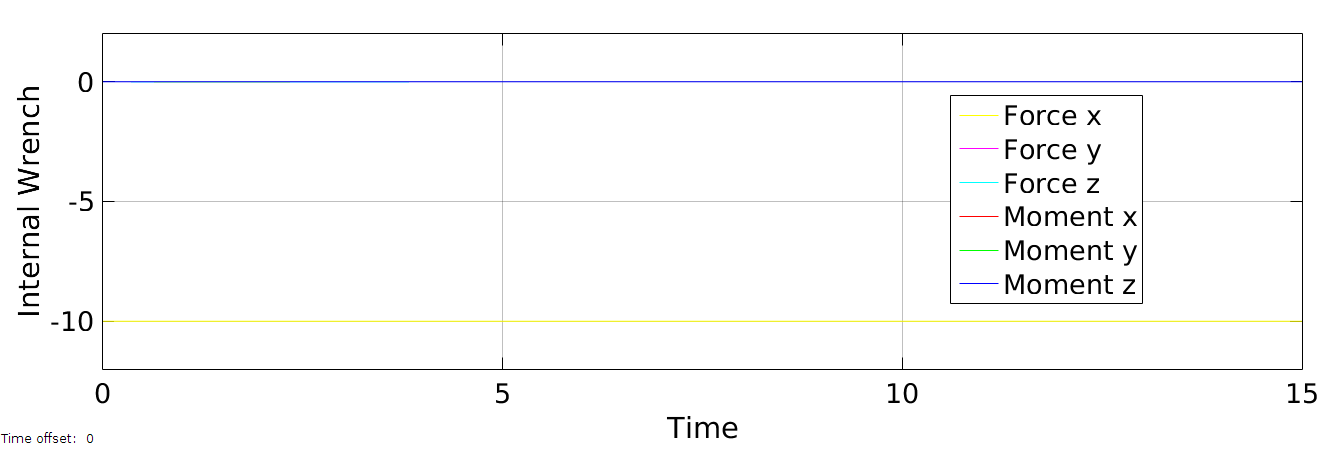
\includegraphics[width=\linewidth]{IntForceStepAllocator}
\caption{Internal wrench for translational motion}
\label{IntForceAllocator}
\end{figure}
\subsection{Constant rotation}  
The object is moved in a sinusoidal velocity curve in x-direction and with constant velocity in z-direction. It is rotated with constant angular velocity in y- and z- direction. Deviations occur in transient behaviour, changing velocity with a step (see figure \ref{IntForceStep}) causes high internal forces in the allocator-free system.
\begin{figure}
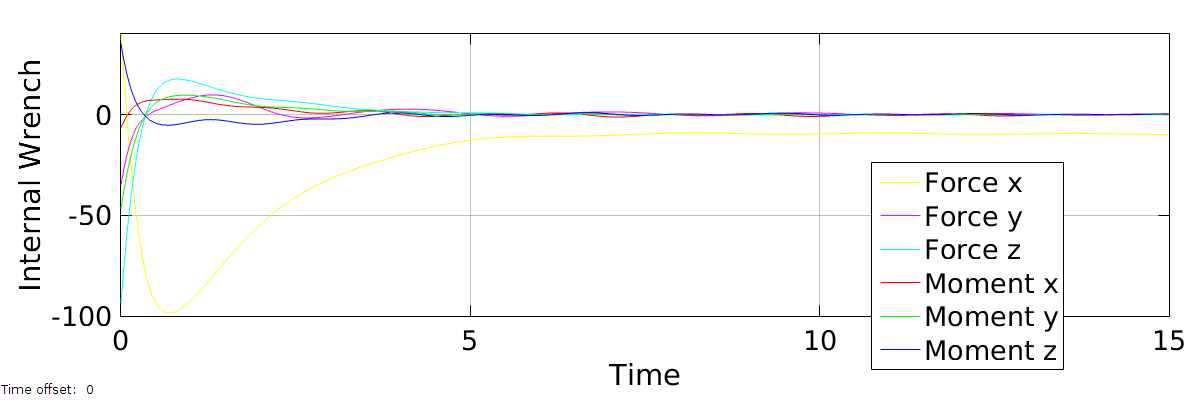
\includegraphics[width=\linewidth]{IntForceStep2}
\caption{Internal wrench for a step in velocity}
\label{IntForceStep}
\end{figure}
 A step is a non-steady function, its derivative (i.e. the acceleration) is infinite. In the simulation, where the derivative is calculated numerically,the step stills results in high accelerations. To avoid this behaviour the step is passed through a first-order (PT1) filter. Figure \ref{IntForcePT1} shows a significant reduction of the internal forces for the smooth input. 
\begin{figure}
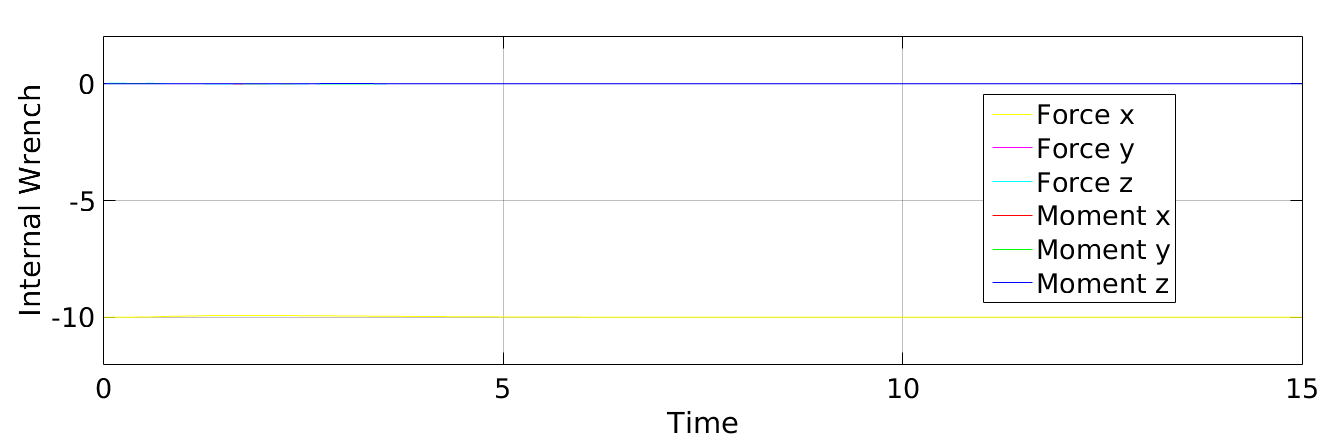
\includegraphics[width=\linewidth]{IntForcePT1}
\caption{Internal wrench for a PT1- filtered step}
\label{IntForcePT1}
\end{figure}
In both cases the internal forces approach their desired values after some time. In steady-state no undesired internal forces are exerted on the object for constant rotation and arbitrary translation. Using the allocator the desired values are set immediately like in the purely translational case.\\
\subsection{Time-variant rotation} 
Main difference to the previous is a permanent and varying angular acceleration of the object. Rotational velocity around the z-axis is given by a \textit{Sinus}-function, for simplicity no further rotation is applied, translational motion leave the internal wrenches unaffected. The lower part of figure \ref{IntForceSinus} shows undamped oscillation in y-direction and around the z-direction, frequency is the equal to the sinusoidal excitation. The upper part shows the desired internal force around in x-direction, accounting for the friction grasp. Constant oscillations with double frequency of the excitation are observed at first, then they are followed by unspecific behaviour. Long time simulations show that constant oscillation alternates with unspecific behaviour,for reasons unknown. Following the theory part, which identifies stiffness as the only possible contributor to internal wrench, stiffness is excluded from the control law. This results in oscillations of increasing amplitude and unstable behaviour. On the contrary simulations show that rotational acceleration induces internal wrench.  
\begin{figure}
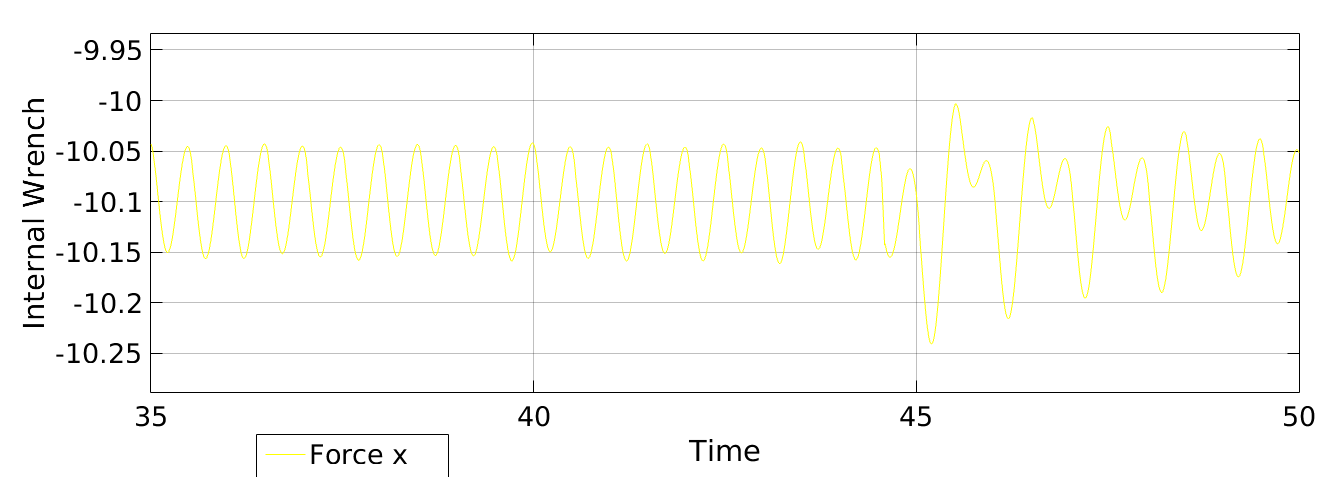
\includegraphics[width=\linewidth]{IntForceSinus2}
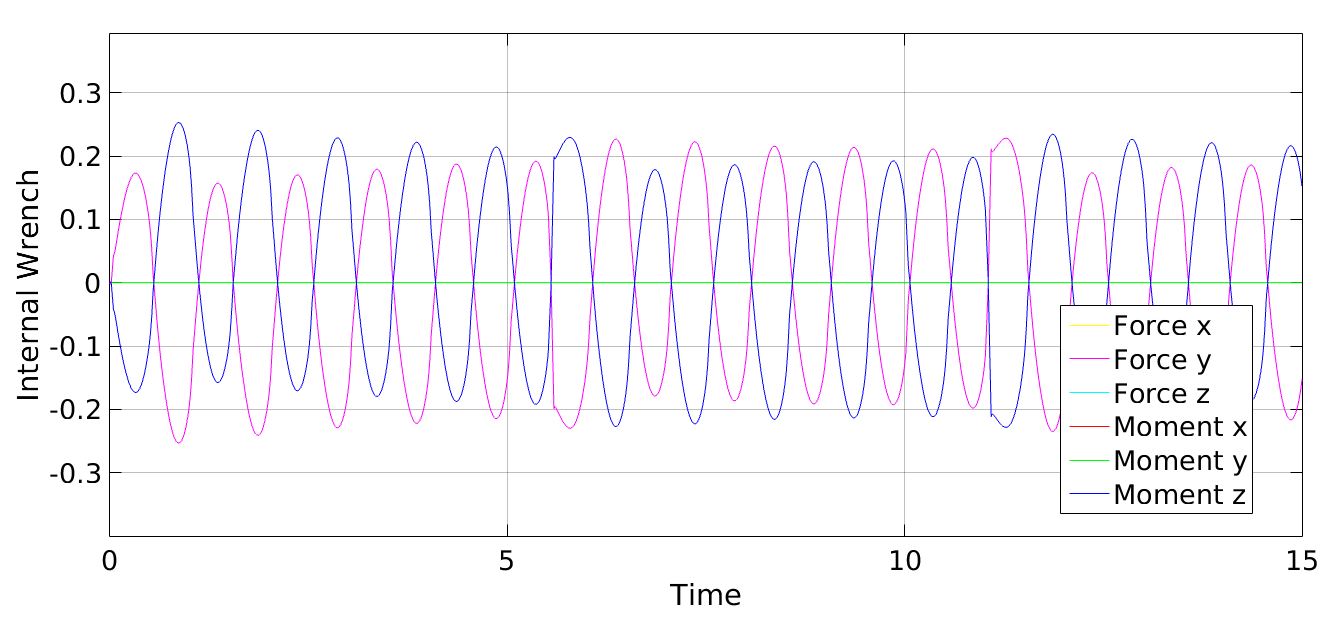
\includegraphics[width=\linewidth]{IntForceSinus1}
\caption{Internal wrench for sinusoidal rotation}
\label{IntForceSinus}
\end{figure} 
Including the allocator exhibits perfect results.
\subsection{Modelling error: Deviation in inertia}
The derivation of the desired forces in the allocator-free approach is only dependent on the grasp geometry. For the allocator manipulator inertia and motion-inducing wrench are also needed. In some cases the manipulator inertia may no exactly be known, and may thus deviate from the apparent inertia. To simulate the influence of uncertainties the inertia used in the allocator and in the impedance control is set to 1.05 of the apparent inertia.\\
For the case of purely translational motion, with or without the allocator no deviations to the desired behaviour can be observed.
Adding constant rotation the steady-state value of the desired internal force decreases uniformly for allocator and non-allocator system. The allocator shows better transient behaviour (see figure \ref{IntDevPT1}).
\begin{figure}
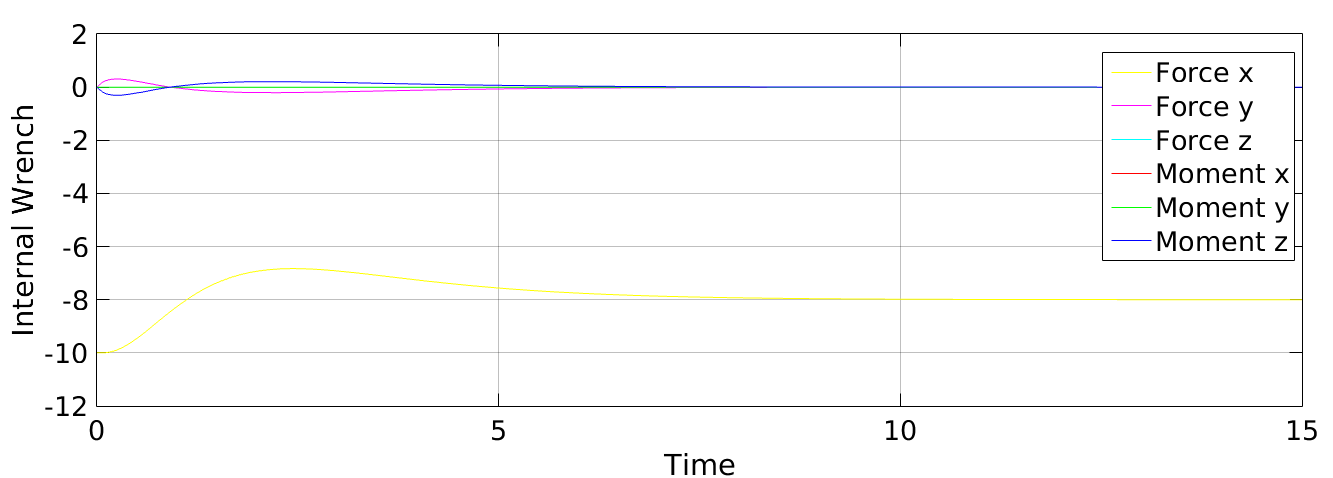
\includegraphics[width=\linewidth]{IntDevNullPT1}
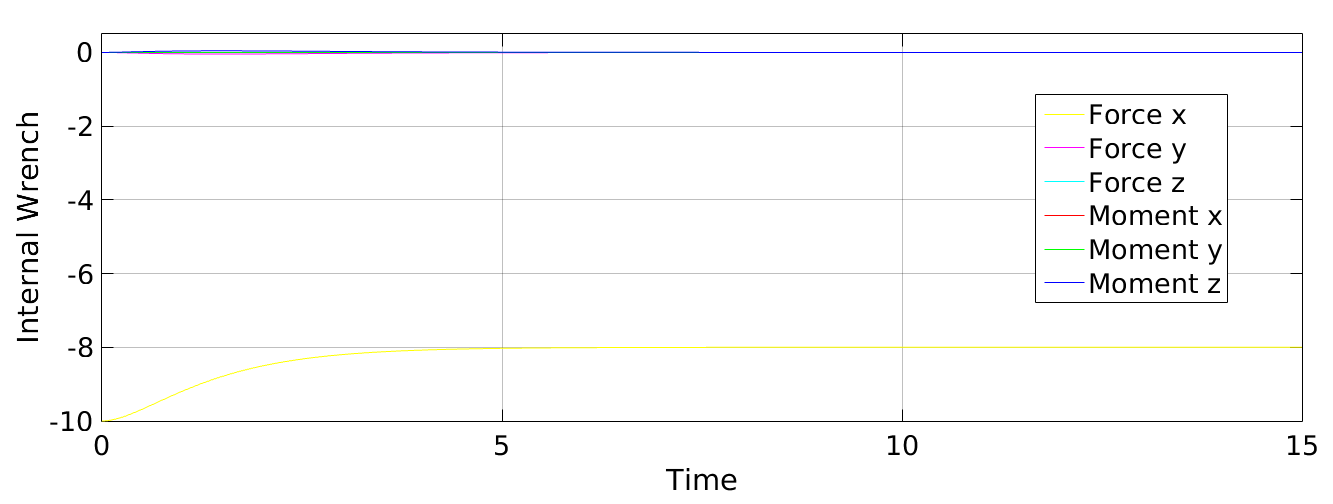
\includegraphics[width=\linewidth]{IntDevAlloPT1}
\caption{Internal wrench for inertia deviation and constant angular velocity with (lower) and without allocator}
\label{IntDevPT1}
\end{figure}
Using sinusoidal rotational velocity both systems show (figure ) oscillations, using the allocator they are smaller.
\begin{figure}
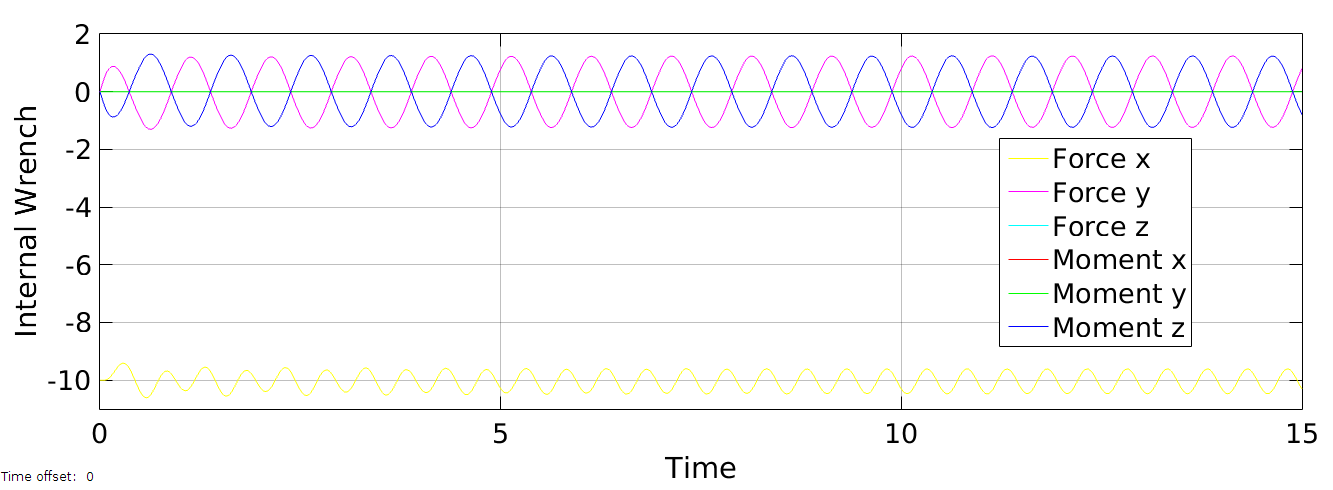
\includegraphics[width=\linewidth]{IntDevNullSinus}
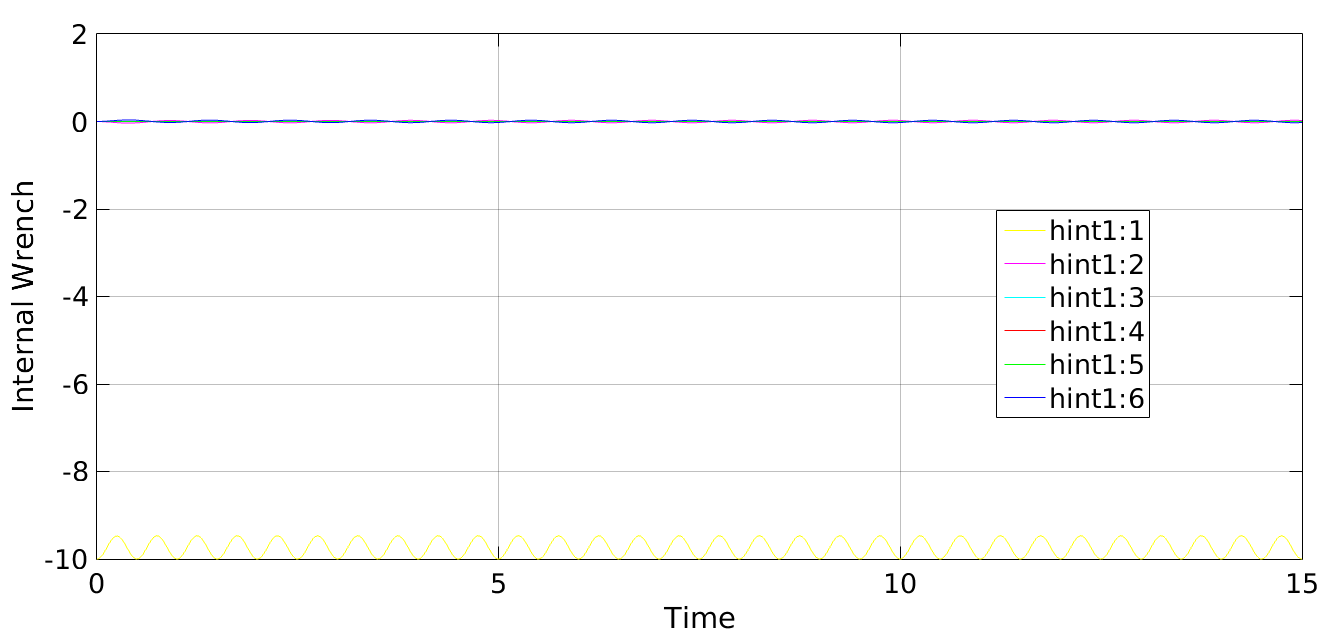
\includegraphics[width=\linewidth]{IntDevAlloSinus}
\caption{Internal wrench for inertia deviation and sinusoidal angular velocity with (lower) and without allocator}
\label{IntDevPT1}
\end{figure}
Even for inertia uncertainties the allocator shows better results than going without it.
\subsection{Time delay in control signals}



\section{Conclusions}








% that's all folks
\end{document}


